\documentclass[mathserif]{beamer}
\usepackage{beamerthemeshadow}
\usepackage{beamerthemesplit}
%\usetheme{shadow}
\usecolortheme{default}
\setbeamertemplate{footline}[frame number]
\useinnertheme[shadow=true]{rounded}
%\setbeamertemplate{footline}{\insertframenumber/\inserttotalframenumber}
%\useoutertheme{infolines}
%\setbeamertemplate{headline}{} % removes the headline that infolines inserts

%\usetheme{boxes}
%\usepackage{amsmass}
%\usepackage{amssymb,amsfonts,url}

\usepackage{algorithm}
\usepackage{algorithmic}

\usepackage{graphicx}
\graphicspath{{Problems/}}

\usepackage{tikz}
\usepackage{pgfplots}

%\usepackage{CJK}
%\usepackage{pinyin}

%    \begin{figure}
%        \centering
%        \includegraphics[width=0.8\textwidth]{newGeneRep.eps}
%    \end{figure}

% \begin{figure}%
%   \begin{center}%
%     \begin{minipage}{0.70\textwidth}%
%      \includegraphics[width=1.0\textwidth]{comp25000.eps}%
%     \end{minipage}%
%     \begin{minipage}{0.30\textwidth}
%      \includegraphics[width=1.0\textwidth]{comparelabel.eps}%
%     \end{minipage}%
%   \end{center}
% \end{figure}

% \begin{table}
%   {\begin{tabular}{l|rrr}\hline
%       & \multicolumn{3}{c}{Actual number of DCJ operations}\\
%       \# genes &\# genes $\times 1$&\# genes $\times 2$&\# genes  $\times 3$ \\
% \hline
%      (a)~25,000 & 0.5\% ~~&  0.9\% ~~& 1.7\%~~\\
%       (b)~10,000 & 0.8\%~~ &  1.4\% ~~& 2.7\%~~\\
%      (c)~ 1,000 & 2.7\%~~ & 4.7\%~~ & 14.7\%~~\\ \hline
%     \end{tabular}} {}%
% \end{table}

% \begin{eqnarray}
% T(n) &=&  \sum_{i=1}^n C_i \\
%      &=&  \# PUSH + \#POP \\
%      &<& 2\times \#PUSH \\
%      &<& 2n \\
% \end{eqnarray}

% \[
% \begin{matrix}
% \begin{pmatrix}
% C_{11} & C_{12} \\
% C_{21} & C_{22}
% \end{pmatrix}
% =
% \begin{pmatrix}
%  \mathbf{a}_{11} &  \mathbf{a}_{12} \\
%  \mathbf{a}_{21} &  \mathbf{a}_{22}
% \end{pmatrix}
%
% \begin{pmatrix}
% B_{11} & B_{12} \\
% B_{21} & B_{22}
%
% \end{pmatrix}
%
%    \end{matrix}
% \]
%
%
% \begin{eqnarray}
%  C_{11} &=& ( \mathbf{a}_{11}\times B_{11}) + ( \mathbf{a}_{12} \times B_{21}) \\
% C_{12} &=& ( \mathbf{a}_{11}\times B_{12}) + ( \mathbf{a}_{12} \times B_{22}) \\
% C_{21} &=& ( \mathbf{a}_{21}\times B_{11}) + ( \mathbf{a}_{22} \times B_{21}) \\
% C_{22} &=& ( \mathbf{a}_{21}\times B_{12}) + ( \mathbf{a}_{22} \times B_{22})
% \end{eqnarray}
% \begin{figure}%
%      \begin{minipage}{0.32\textwidth}%
%       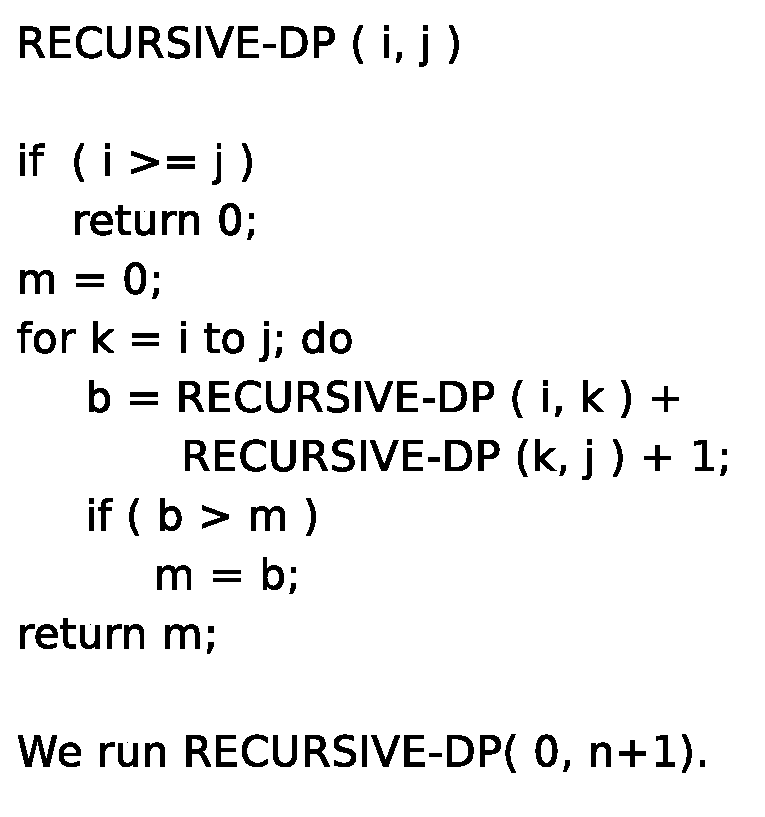
\includegraphics[width=1.0\textwidth]{L7-intervalschedulingdpalgo.eps}%
%      \end{minipage}%
%  \quad
%      \begin{minipage}{0.30\textwidth}
%       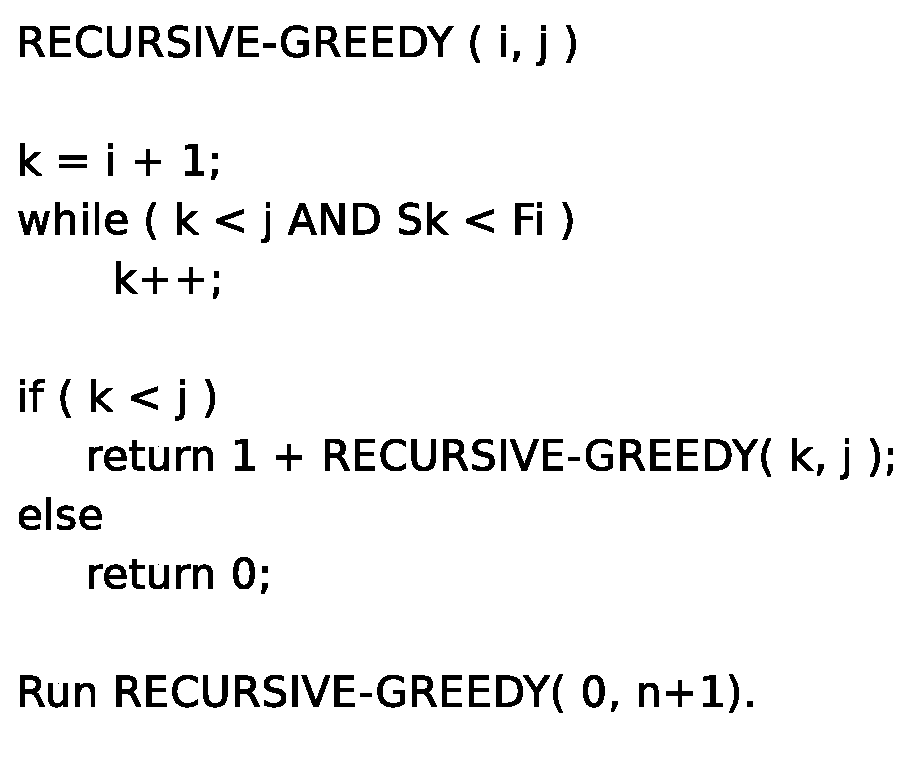
\includegraphics[width=1.0\textwidth]{L7-intervalschedulinggreedyalgo.eps}%
%      \end{minipage}%
%  \quad
%       \begin{minipage}{0.25\textwidth}
%       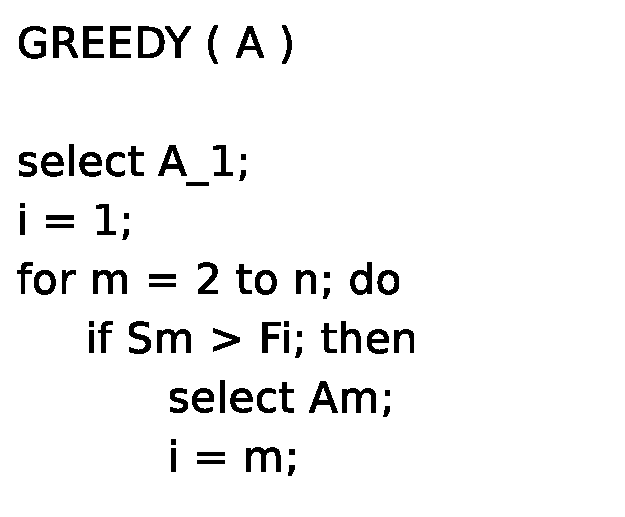
\includegraphics[width=1.0\textwidth]{L7-intervalschedulinggreedyalgo2.eps}%
%      \end{minipage}%
%
%  \end{figure}

\title{CS711008Z  Algorithm Design and Analysis }
\subtitle{ Lecture 8. An example of cycling in simplex algorithm}
\author{Dongbo Bu }
\institute{ {\small Institute of Computing Technology \\
Chinese Academy of Sciences, Beijing, China}}

\date{}

\begin{document}
%\begin{CJK}{UTF8}{cyberbit}

\frame{\titlepage}



\frame{
\begin{block}{}
Cycling in simplex algorithm
\end{block}
}

\frame{
	\begin{itemize}
		\item  
Cycling: If a sequence of pivots starting from some basic feasible solution ends up at the exact same basic feasible solution, then we refer to this as “cycling.” If the simplex method cycles, it can cycle forever.
		\item In 1953, Hoffman gave the first cycling example, which had 11 variables and 3 equations. 
		\item In 1955, E. M. L. Beale gave a smaller example, which had 7 variables and 3 equations. 
	\end{itemize}

	
}

\frame{


Standard form:

\[
\begin{array}{rrrrrrrrrrrrrrrrl}
 \min & -\frac{3}{4} x_1     &+&  150 x_2   &-&\frac{1}{50} x_3  &+& 6x_4  & & \\
 s.t. &   \frac{1}{4}x_1       &-&   60  x_2    &-& \frac{1}{25} x_3  &+& 9x_4					& \leq & 0   \\
      &   \frac{1}{2}x_1      &-&    90 x_2      &-& \frac{1}{50} x_3  &+& 3x_4 					& \leq & 0   \\
      &                              & &                     & &  x_3		       & &						& \leq & 1   \\
      &   x_1                     &,&   x_2           &,&  x_3	               &,& x_4					& \geq & 0   \\
\end{array} \nonumber
\]

Slack form:
\[
\begin{array}{rrrrrrrrrrrrrrrrrrrrrl}
 \min & -\frac{3}{4} x_1     &+  150 x_2   &-\frac{1}{50} x_3  &+ 6x_4 &  &  & &  &  \\
 s.t. &   \frac{1}{4}x_1       &-   60  x_2    &- \frac{1}{25} x_3  &+ 9x_4	&+x_5 &   &  &				& \leq & 0   \\
      &   \frac{1}{2}x_1      &-    90 x_2      &- \frac{1}{50} x_3  &+ 3x_4 	&   &+x_6	 &  &			& \leq & 0   \\
      &           &             & &  x_3		& 						&   & +&x_7				& \leq & 1   \\
      &   x_1     &,   x_2      &,  x_3	&, x_4	&  &  &  							& \geq & 0   \\
\end{array} \nonumber
\]

}


\frame{
\frametitle{ Step 1. }

%\begin{figure}
% 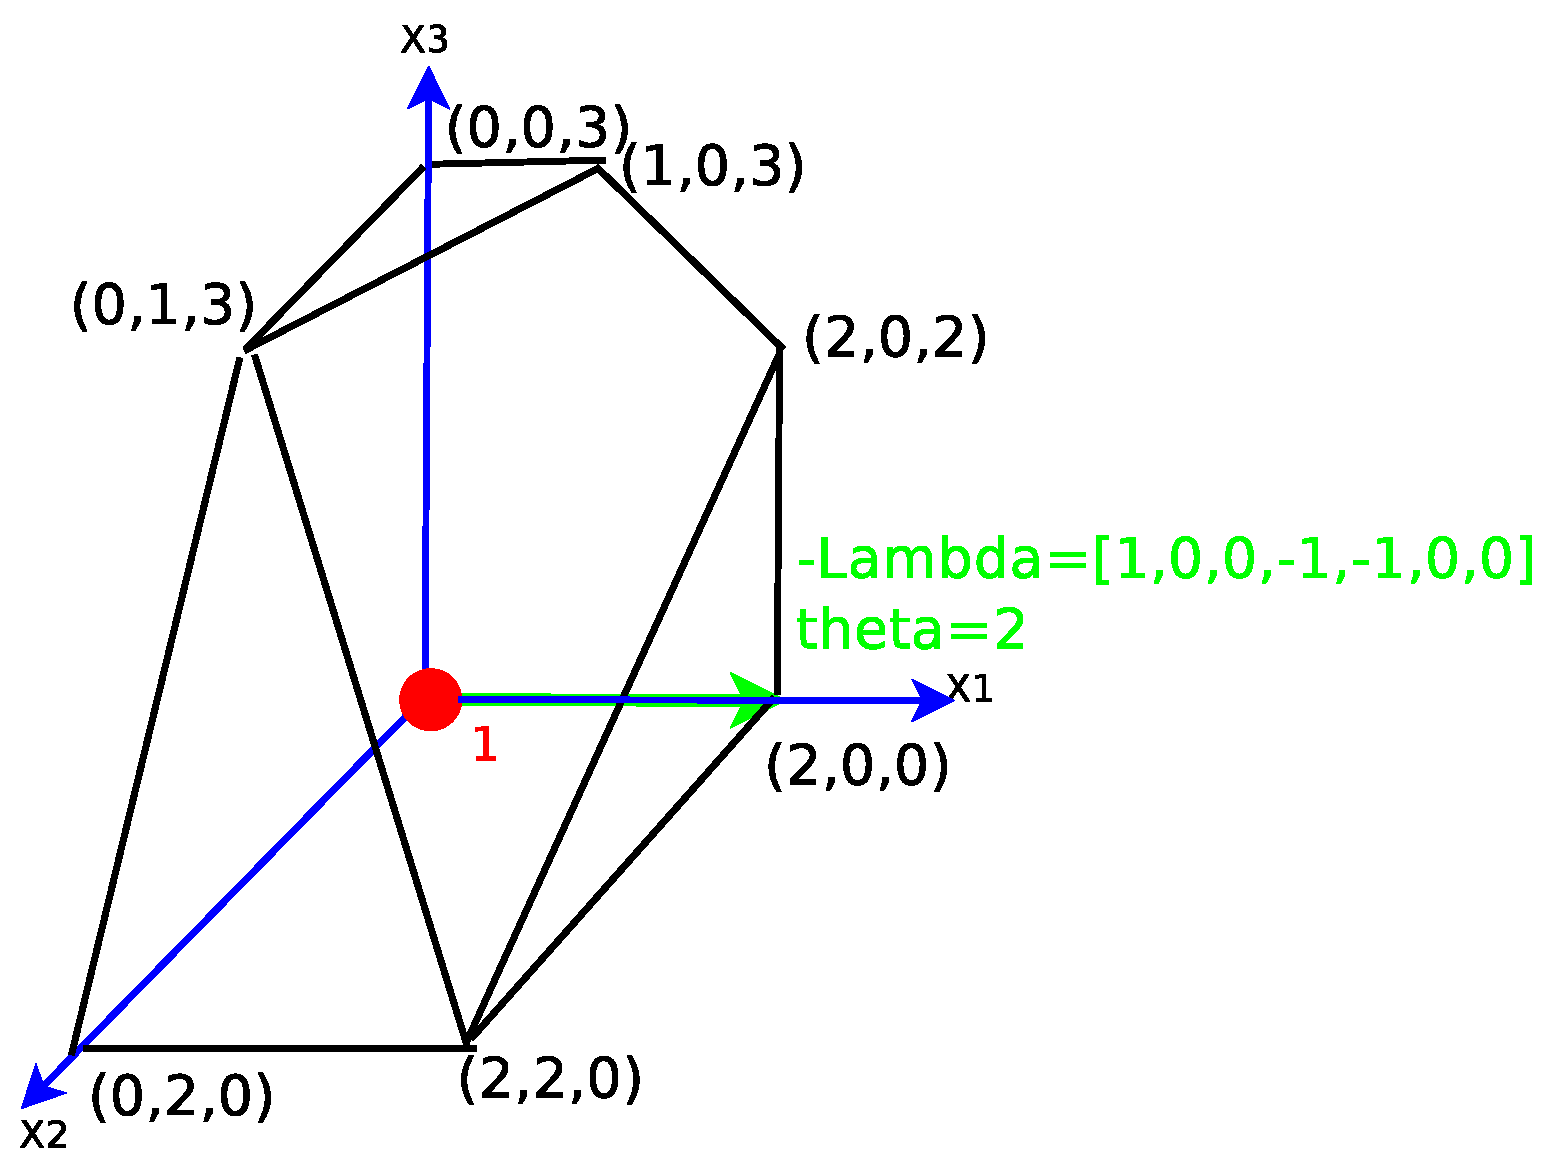
\includegraphics[width=1.4in] {L8-LPexample3Dstep1.eps}
%\end{figure}


\begin{small}
\begin{table}
{
\begin{tabular}{r|rrrrrrr}\hline 
  & $x_1$ & $x_2$ & $x_3$ & {$x_4$} & \textcolor{blue}{$x_5$} & \textcolor{blue}{$x_6$} & \textcolor{blue}{$x_7$}\\
\hline
 -z= 0 & $\overline{c_1}$=$-\frac{3}{4}$ & $\overline{c_2}$=150 & $\overline{c_3}$=$-\frac{1}{50}$ & $\overline{c_4}$=6 & $\overline{c_5}$=0 & $\overline{c_6}$=0 & $\overline{c_7}$=0 \\
 \hline
 $\mathbf{x_{B1}} = b_1'$=0 & \textcolor{red}{$\frac{1}{4}$} & -60 & $-\frac{1}{25}$ & 9 & \textcolor{blue}{1} & \textcolor{blue}{0} & \textcolor{blue}{0} \\
 $\mathbf{x_{B2}} = b_2'$=0 &  $\frac{1}{2}$ & -90 & $-\frac{1}{50}$ & 3 &  \textcolor{blue}{0}  &  \textcolor{blue}{1} & \textcolor{blue}{0} \\
 $\mathbf{x_{B3}} = b_3'$=1 &  0 & 0 & 1 & 0 &  \textcolor{blue}{0} & \textcolor{blue}{0} & \textcolor{blue}{1} \\
\hline
\end{tabular}
} %{}%
\end{table}
\end{small}

\begin{itemize}
 \item Basis (in blue): $\mathbf{B =\{ a_5, a_6, a_7 \} }$.
 \item Solution: $\mathbf{x = [ x_B, x_N ] = [ B^{-1}b, 0] }= [ 0, 0, 0, 0, 0, 0, 1 ]$. 
 \item Pivoting (in red): choose $\mathbf{a_1}$ to enter basis since $\overline{c_1} = -\frac{3}{4} < 0$; choose $\mathbf{a_5}$ to 
 exit since $\theta = \min_{\mathbf{a}_i \in \mathbf{B}, \lambda_{i}>0} \frac{b'_i}{\lambda_{i} } = \frac{b'_1}{\lambda_{1} }= 0$.
     \item Here, the corresponding $\mathbf{\lambda}$ is stored in the $1$-st column (Why? the basis $\mathbf{B}$ forms an identity matrix.)
\end{itemize}


}



\frame{
\frametitle{ Step 2. }

%\begin{figure}
% 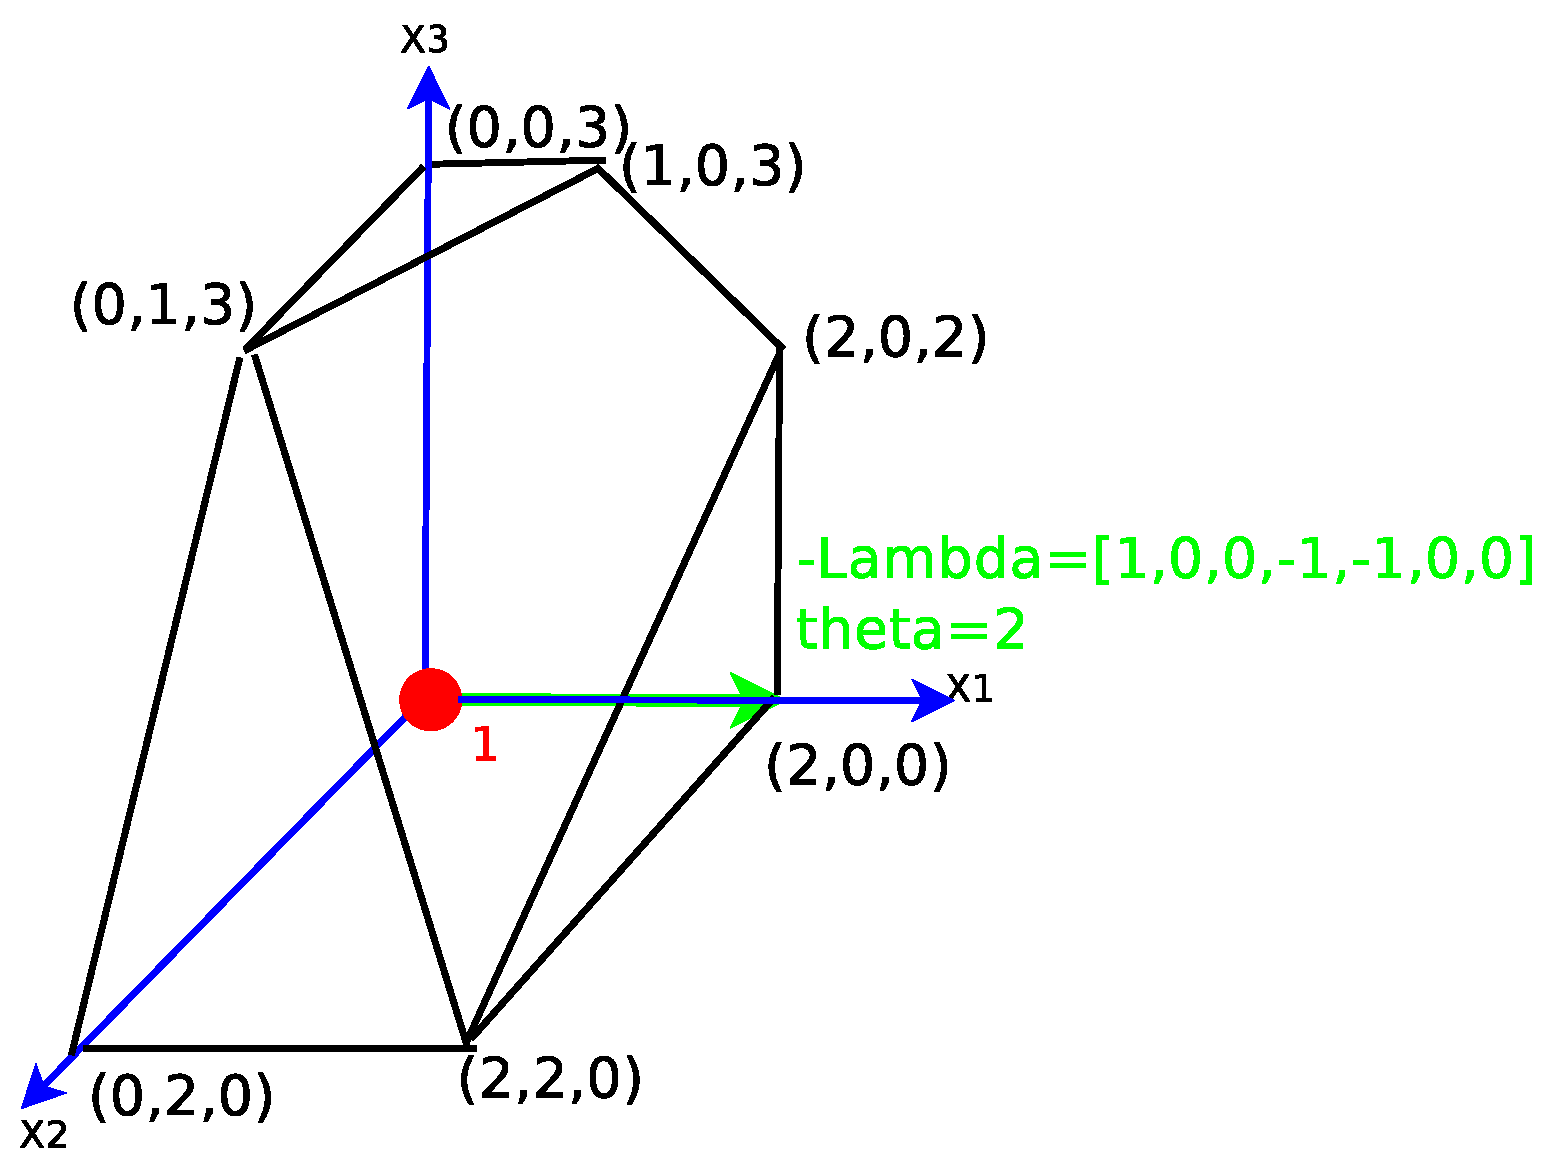
\includegraphics[width=1.4in] {L8-LPexample3Dstep1.eps}
%\end{figure}


\begin{small}
\begin{table}
{
\begin{tabular}{r|rrrrrrr}\hline 
  & $\textcolor{blue}{x_1}$ & $x_2$ & $x_3$ & {$x_4$} & \textcolor{black}{$x_5$} & \textcolor{blue}{$x_6$} & \textcolor{blue}{$x_7$}\\
\hline
 -z= 0 & $\overline{c_1}$=0 & $\overline{c_2}$=-30 & $\overline{c_3}$=$-\frac{7}{50}$ & $\overline{c_4}$=33 & $\overline{c_5}$=3 & $\overline{c_6}$=0 & $\overline{c_7}$=0 \\
 \hline
 $\mathbf{x_{B1}} = b_1'$=0 & \textcolor{blue}{1} & -240 & $-\frac{4}{25}$ & 36 & {4} & \textcolor{blue}{0} & \textcolor{blue}{0} \\
 $\mathbf{x_{B2}} = b_2'$=0 &  \textcolor{blue}{0} & \textcolor{red}{30} & $\frac{3}{50}$ & -15 &  -2  &  \textcolor{blue}{1} & \textcolor{blue}{0} \\
 $\mathbf{x_{B3}} = b_3'$=1 &  \textcolor{blue}{0} & 0 & 1 & 0 &  0 & \textcolor{blue}{0} & \textcolor{blue}{1} \\
\hline
\end{tabular}
} %{}%
\end{table}
\end{small}

\begin{itemize}
 \item Basis (in blue): $\mathbf{B =\{ a_1, a_6, a_7 \} }$.
 \item Solution: $\mathbf{x = [ x_B, x_N ] = [ B^{-1}b, 0] }= [ 0, 0, 0, 0, 0, 0, 1 ]$. 

 \item Pivoting (in red): choose $\mathbf{a_2}$ to enter basis since $\overline{c_2} = -30 < 0$; choose $\mathbf{a_6}$ to exit 
 since $\theta = \min_{\mathbf{a}_i \in \mathbf{B}, \lambda_{i}>0} \frac{b'_i}{\lambda_{i} } = \frac{b'_2}{\lambda_{2} }= 0$.
     \item Here, the corresponding $\mathbf{\lambda}$ is stored in the $2$-nd column (Why? the basis $\mathbf{B}$ forms an identity matrix.)
\end{itemize}

}



\frame{
\frametitle{ Step 3. }

%\begin{figure}
% 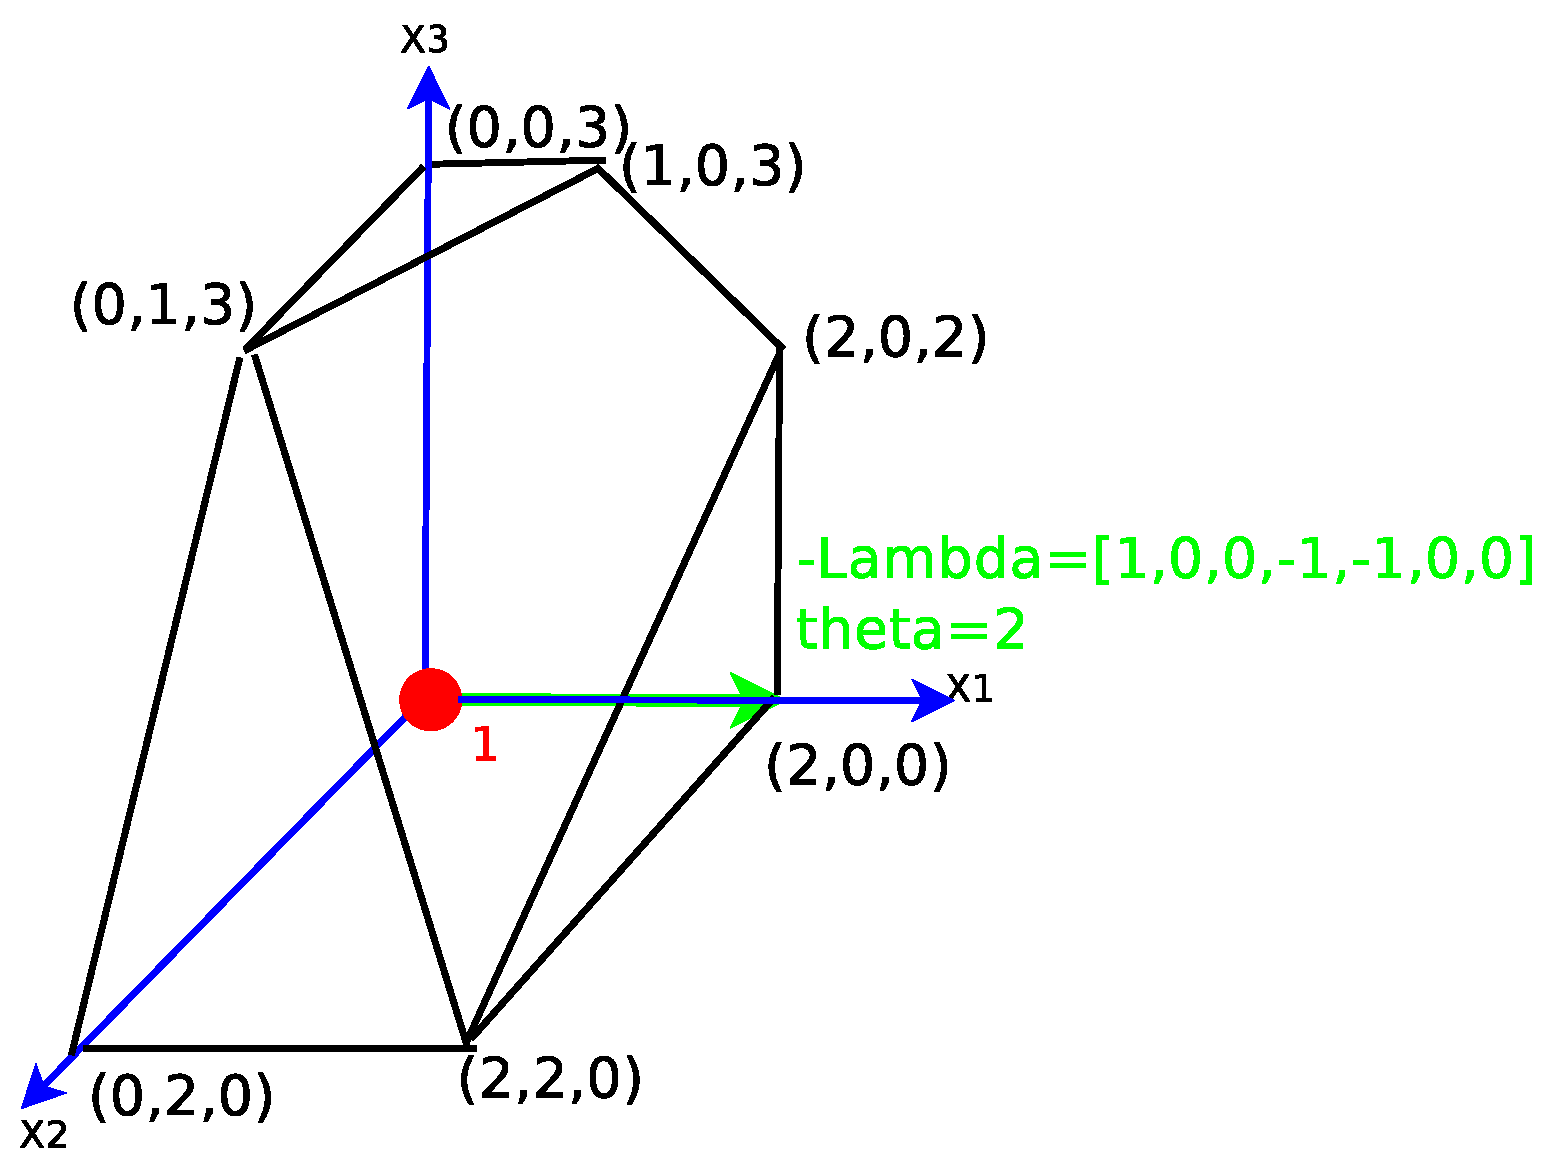
\includegraphics[width=1.4in] {L8-LPexample3Dstep1.eps}
%\end{figure}


\begin{small}
\begin{table}
{
\begin{tabular}{r|rrrrrrr}\hline 
  & $\textcolor{blue}{x_1}$ & $\textcolor{blue}{x_2}$ & $x_3$ & {$x_4$} & \textcolor{black}{$x_5$} & \textcolor{black}{$x_6$} & \textcolor{blue}{$x_7$}\\
\hline
 
 -z= 0 & $\overline{c_1}$=0 & $\overline{c_2}$=0 & $\overline{c_3}$=$-\frac{2}{25}$ & $\overline{c_4}$=18 & $\overline{c_5}$=1 & $\overline{c_6}$=1 & $\overline{c_7}$=0 \\
 \hline
 
 $\mathbf{x_{B1}} = b_1'$=0 & \textcolor{blue}{1} & \textcolor{blue}{0} & \textcolor{red}{$\frac{8}{25}$} & -84 & -12 & 8 & \textcolor{blue}{0} \\
 
 $\mathbf{x_{B2}} = b_2'$=0 &  \textcolor{blue}{0} & \textcolor{blue}{1} & $\frac{1}{500}$ & -$\frac{1}{2}$ & $-\frac{1}{15}$  &  $\frac{1}{30}$& \textcolor{blue}{0} \\
 
 $\mathbf{x_{B3}} = b_3'$=1 &  \textcolor{blue}{0} &  \textcolor{blue}{0} & 1 & 0 &  0 &0 & \textcolor{blue}{1} \\
\hline
\end{tabular}
} %{}%
\end{table}
\end{small}

\begin{itemize}
 \item Basis (in blue): $\mathbf{B =\{ a_1, a_2, a_7 \} }$.
 \item Solution: $\mathbf{x = [ x_B, x_N ] = [ B^{-1}b, 0] }= [ 0, 0, 0, 0, 0, 0, 1 ]$. 

 \item Pivoting (in red): choose $\mathbf{a_3}$ to enter basis since $\overline{c_3} = -\frac{2}{25} < 0$; 
 choose $\mathbf{a_1}$ to exit since $\theta = \min_{\mathbf{a}_i \in \mathbf{B}, \lambda_{i}>0} \frac{b'_i}{\lambda_{i} } = \frac{b'_1}{\lambda_{1} }= 0$.
     \item Here, the corresponding $\mathbf{\lambda}$ is stored in the $3$-rd column (Why? the basis $\mathbf{B}$ forms an identity matrix.)
\end{itemize}

}



\frame{
\frametitle{ Step 4. }

%\begin{figure}
% 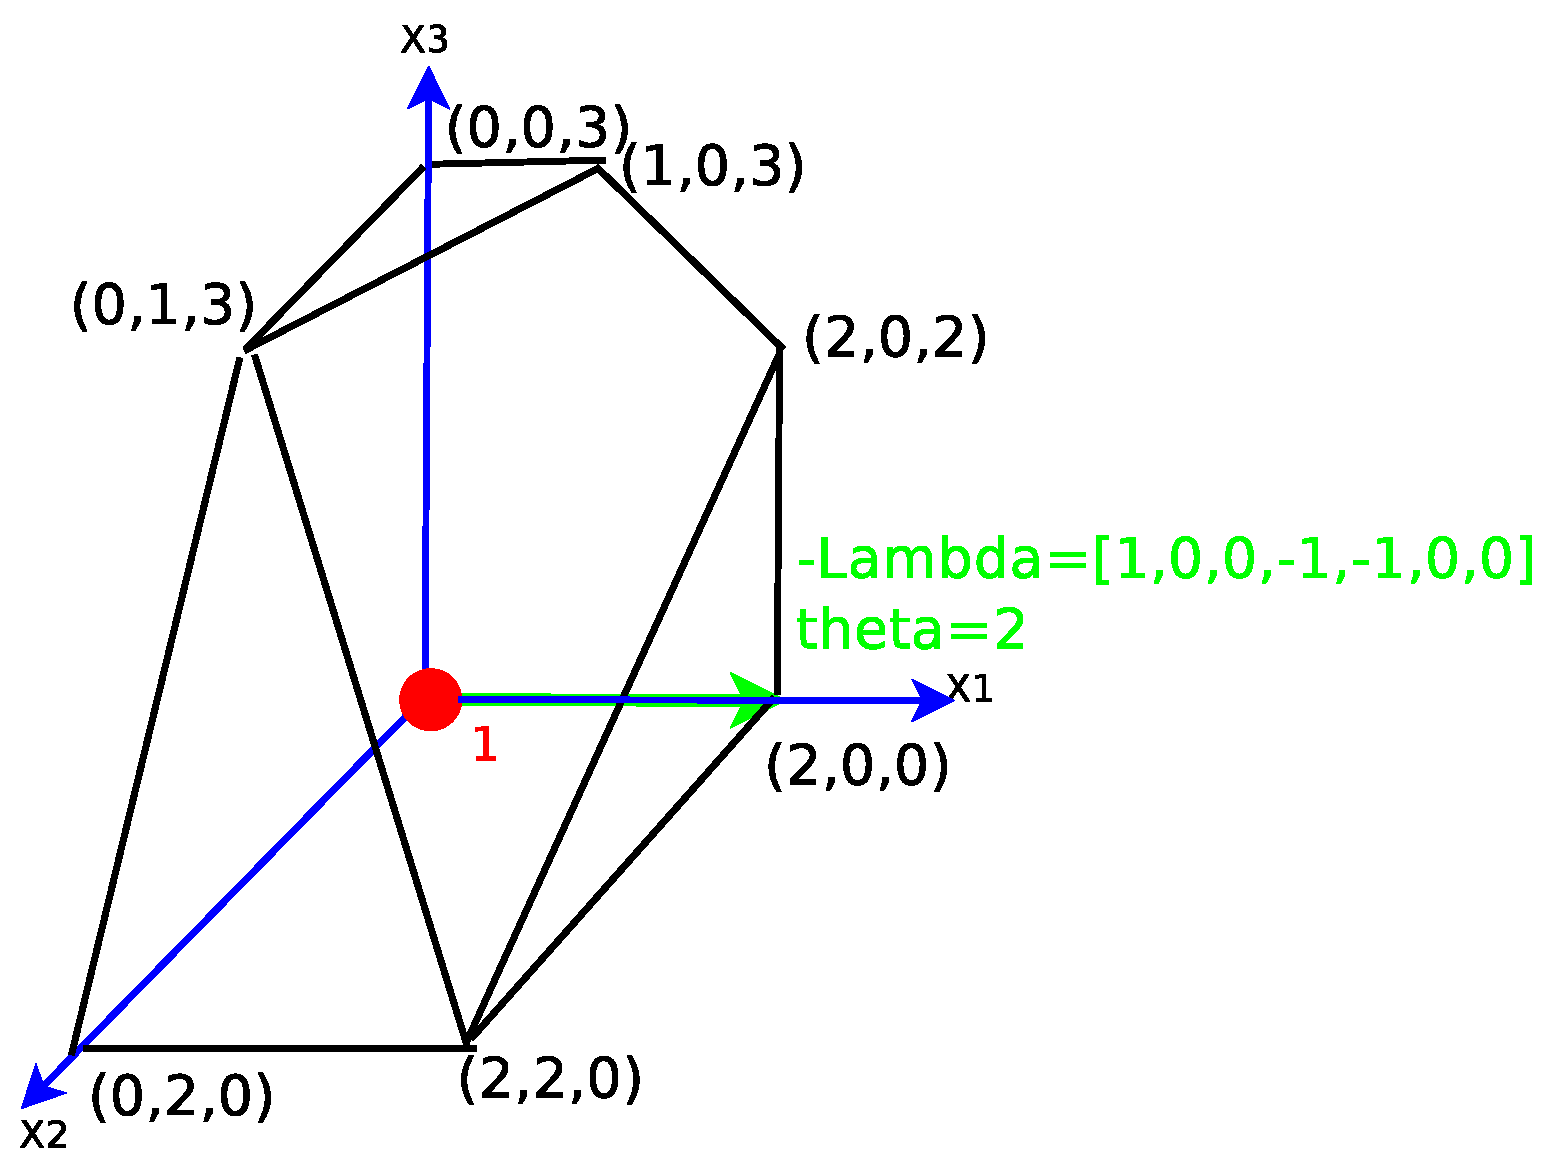
\includegraphics[width=1.4in] {L8-LPexample3Dstep1.eps}
%\end{figure}


\begin{small}
\begin{table}
{
\begin{tabular}{r|rrrrrrr}\hline 
  & $\textcolor{black}{x_1}$ & $\textcolor{blue}{x_2}$ & $\textcolor{blue}{x_3}$  & {$x_4$} & \textcolor{black}{$x_5$} & \textcolor{black}{$x_6$} & \textcolor{blue}{$x_7$}\\
\hline
 
 -z= 0 & $\overline{c_1}$=$\frac{1}{4}$ & $\overline{c_2}$=0 & $\overline{c_3}$=0 & $\overline{c_4}$=-3 & $\overline{c_5}$=-2 & $\overline{c_6}$=3 & $\overline{c_7}$=0 \\
 \hline
 
 $\mathbf{x_{B1}} = b_1'$=0 & $\frac{25}{8}$ & \textcolor{blue}{0}    & \textcolor{blue}{1} & $-\frac{525}{2}$ & $-\frac{75}{2}$   & 25 & \textcolor{blue}{0} \\
 
 $\mathbf{x_{B2}} = b_2'$=0 &  $-\frac{1}{60}$  & \textcolor{blue}{1} & \textcolor{blue}{0} & \textcolor{red}{ $\frac{1}{40}$ }   & $\frac{1}{120}$  &  $-\frac{1}{60}$& \textcolor{blue}{0} \\
 
 $\mathbf{x_{B3}} = b_3'$=1 &  $-\frac{25}{8}$ &  \textcolor{blue}{0} & \textcolor{blue}{0} & $\frac{525}{2}$  &  $\frac{75}{2}$   & -25 & \textcolor{blue}{1} \\
\hline
\end{tabular}
} %{}%
\end{table}
\end{small}
\begin{itemize}
 \item Basis (in blue): $\mathbf{B =\{ a_2, a_3, a_7 \} }$.
 \item Solution: $\mathbf{x = [ x_B, x_N ] = [ B^{-1}b, 0] }= [ 0, 0, 0, 0, 0, 0, 1 ]$. 
 \item Pivoting (in red): choose $\mathbf{a_4}$ to enter basis since $\overline{c_4} = -3 < 0$; 
 choose $\mathbf{a_2}$ to exit since $\theta = \min_{\mathbf{a}_i \in \mathbf{B}, \lambda_{i}>0} \frac{b'_i}{\lambda_{i} } = \frac{b'_2}{\lambda_{2} }= 0$.
     \item Here, the corresponding $\mathbf{\lambda}$ is stored in the $4$-th column (Why? the basis $\mathbf{B}$ forms an identity matrix.)
\end{itemize}

}



\frame{
\frametitle{ Step 5. }

%\begin{figure}
% 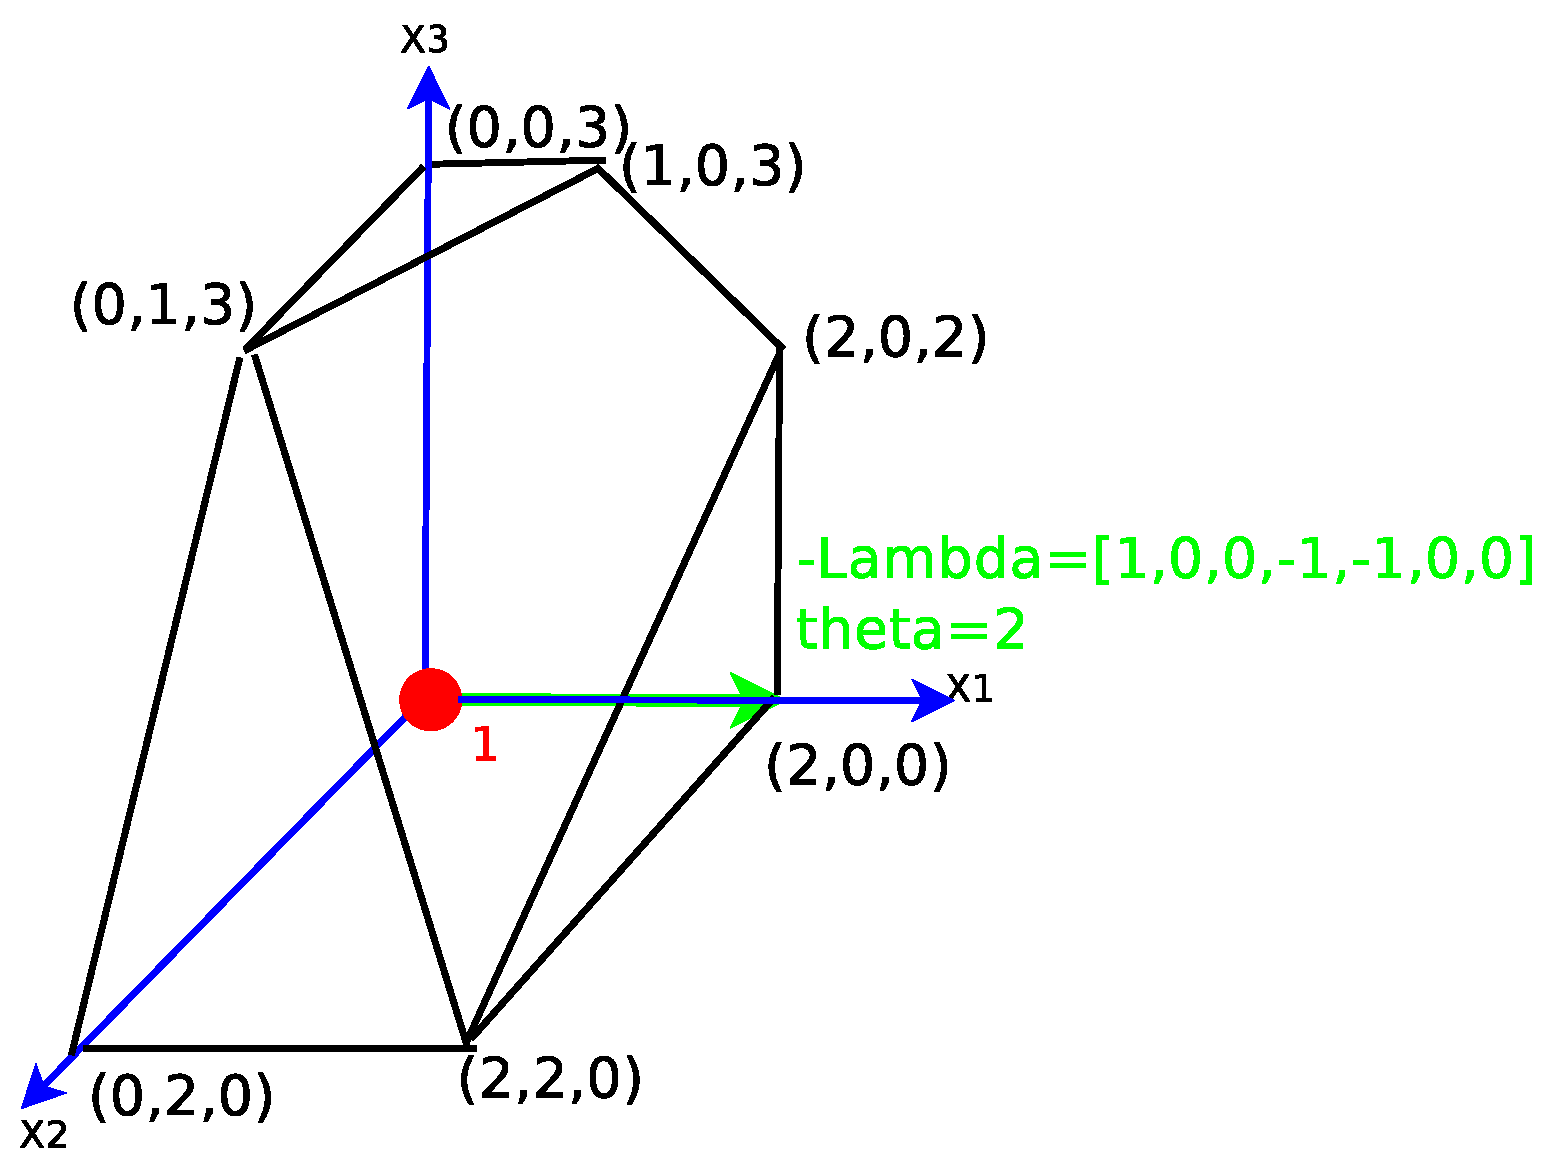
\includegraphics[width=1.4in] {L8-LPexample3Dstep1.eps}
%\end{figure}


\begin{small}
\begin{table}
{
\begin{tabular}{r|rrrrrrr}\hline 
  & $\textcolor{black}{x_1}$ & $\textcolor{black}{x_2}$ & $\textcolor{blue}{x_3}$  & \textcolor{blue}{$x_4$} & \textcolor{black}{$x_5$} & \textcolor{black}{$x_6$} & \textcolor{blue}{$x_7$}\\
\hline
 
 -z= 0 & $\overline{c_1}$=$-\frac{1}{2}$ & $\overline{c_2}$=120 & $\overline{c_3}$=0 & $\overline{c_4}$=0 & $\overline{c_5}$=-1 & $\overline{c_6}$=1 & $\overline{c_7}$=0 \\
 \hline
 
 $\mathbf{x_{B1}} = b_1'$=0 & $-\frac{125}{2}$ & 10500    & \textcolor{blue}{1} &  \textcolor{blue}{0}  & \textcolor{red}{50}   & -150 & \textcolor{blue}{0} \\
 
 $\mathbf{x_{B2}} = b_2'$=0 &  $-\frac{1}{4}$  & 40 & \textcolor{blue}{0} &  \textcolor{blue}{1}    & $\frac{1}{3}$  &  $-\frac{2}{3}$& \textcolor{blue}{0} \\
 
 $\mathbf{x_{B3}} = b_3'$=1 &  $\frac{125}{2}$ & 10500 & \textcolor{blue}{0} &  \textcolor{blue}{0}   &  50   & 150 & \textcolor{blue}{1} \\
\hline
\end{tabular}
} %{}%
\end{table}
\end{small}

\begin{itemize}
 \item Basis (in blue): $\mathbf{B =\{ a_3, a_4, a_7 \} }$.
 \item Solution: $\mathbf{x = [ x_B, x_N ] = [ B^{-1}b, 0] }= [ 0, 0, 0, 0, 0, 0, 1 ]$. 
 \item Pivoting (in red): choose $\mathbf{a_5}$ to enter basis since $\overline{c_5} = -1 < 0$; 
 choose $\mathbf{a_3}$ to exit since $\theta = \min_{\mathbf{a}_i \in \mathbf{B}, \lambda_{i}>0} \frac{b'_i}{\lambda_{i} } = \frac{b'_1}{\lambda_{1} }= 0$.
     \item Here, the corresponding $\mathbf{\lambda}$ is stored in the $5$-th column (Why? the basis $\mathbf{B}$ forms an identity matrix.)
\end{itemize}

}




\frame{
\frametitle{ Step 6. }

%\begin{figure}
% 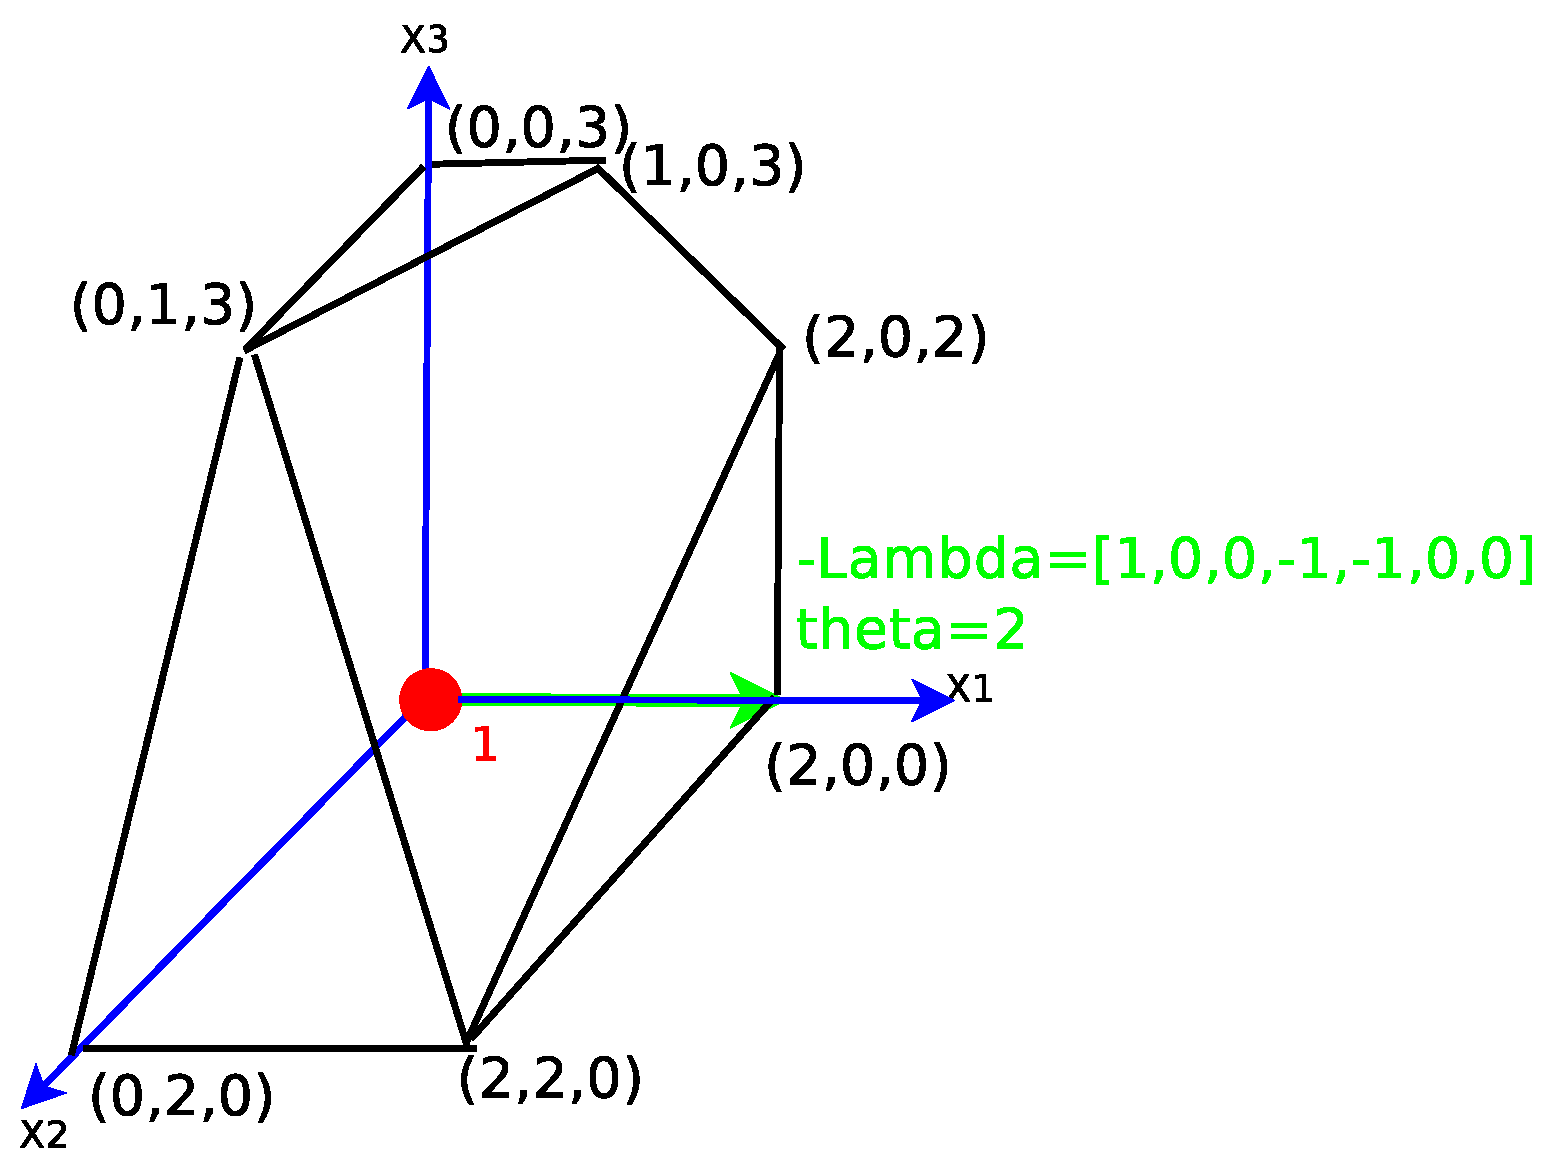
\includegraphics[width=1.4in] {L8-LPexample3Dstep1.eps}
%\end{figure}


\begin{small}
\begin{table}
{
\begin{tabular}{r|rrrrrrr}\hline 
  & $\textcolor{black}{x_1}$ & $\textcolor{black}{x_2}$ & $\textcolor{black}{x_3}$  & \textcolor{blue}{$x_4$} & \textcolor{blue}{$x_5$} & \textcolor{black}{$x_6$} & \textcolor{blue}{$x_7$}\\
\hline
 
 -z= 0 & $\overline{c_1}$=$-\frac{7}{4}$ & $\overline{c_2}$=330 & $\overline{c_3}$=$\frac{1}{50}$ & $\overline{c_4}$=0 & $\overline{c_5}$=0 & $\overline{c_6}$=-2 & $\overline{c_7}$=0 \\
 \hline
 
 $\mathbf{x_{B1}} = b_1'$=0 & $-\frac{5}{4}$ & 210    &  $\frac{1}{50}$ &  \textcolor{blue}{0}  & \textcolor{blue}{1} & -3 & \textcolor{blue}{0} \\
 
 $\mathbf{x_{B2}} = b_2'$=0 &  $\frac{1}{6}$  & -30 & $-\frac{1}{150}$ &  \textcolor{blue}{1}    &  \textcolor{blue}{0} &  \textcolor{red}{$\frac{1}{3}$} & \textcolor{blue}{0} \\
 
 $\mathbf{x_{B3}} = b_3'$=1 &  $ 0 $ & 0  &1                                             &  \textcolor{blue}{0}   &  \textcolor{blue}{0}   & 0 & \textcolor{blue}{1} \\
\hline
\end{tabular}
} %{}%
\end{table}
\end{small}

\begin{itemize}
 \item Basis (in blue): $\mathbf{B =\{ a_4, a_5, a_7 \} }$.
 \item Solution: $\mathbf{x = [ x_B, x_N ] = [ B^{-1}b, 0] }= [ 0, 0, 0, 0, 0, 0, 1 ]$. 
 \item Pivoting (in red): choose $\mathbf{a_6}$ to enter basis since $\overline{c_6} = -2 < 0$; 
 choose $\mathbf{a_4}$ to exit since $\theta = \min_{\mathbf{a}_i \in \mathbf{B}, \lambda_{i}>0} \frac{b'_i}{\lambda_{i} } = \frac{b'_2}{\lambda_{2} }= 0$.
     \item Here, the corresponding $\mathbf{\lambda}$ is stored in the $6$-th column (Why? the basis $\mathbf{B}$ forms an identity matrix.)
\end{itemize}

}

\frame{
\frametitle{ Step 7. }

%\begin{figure}
% 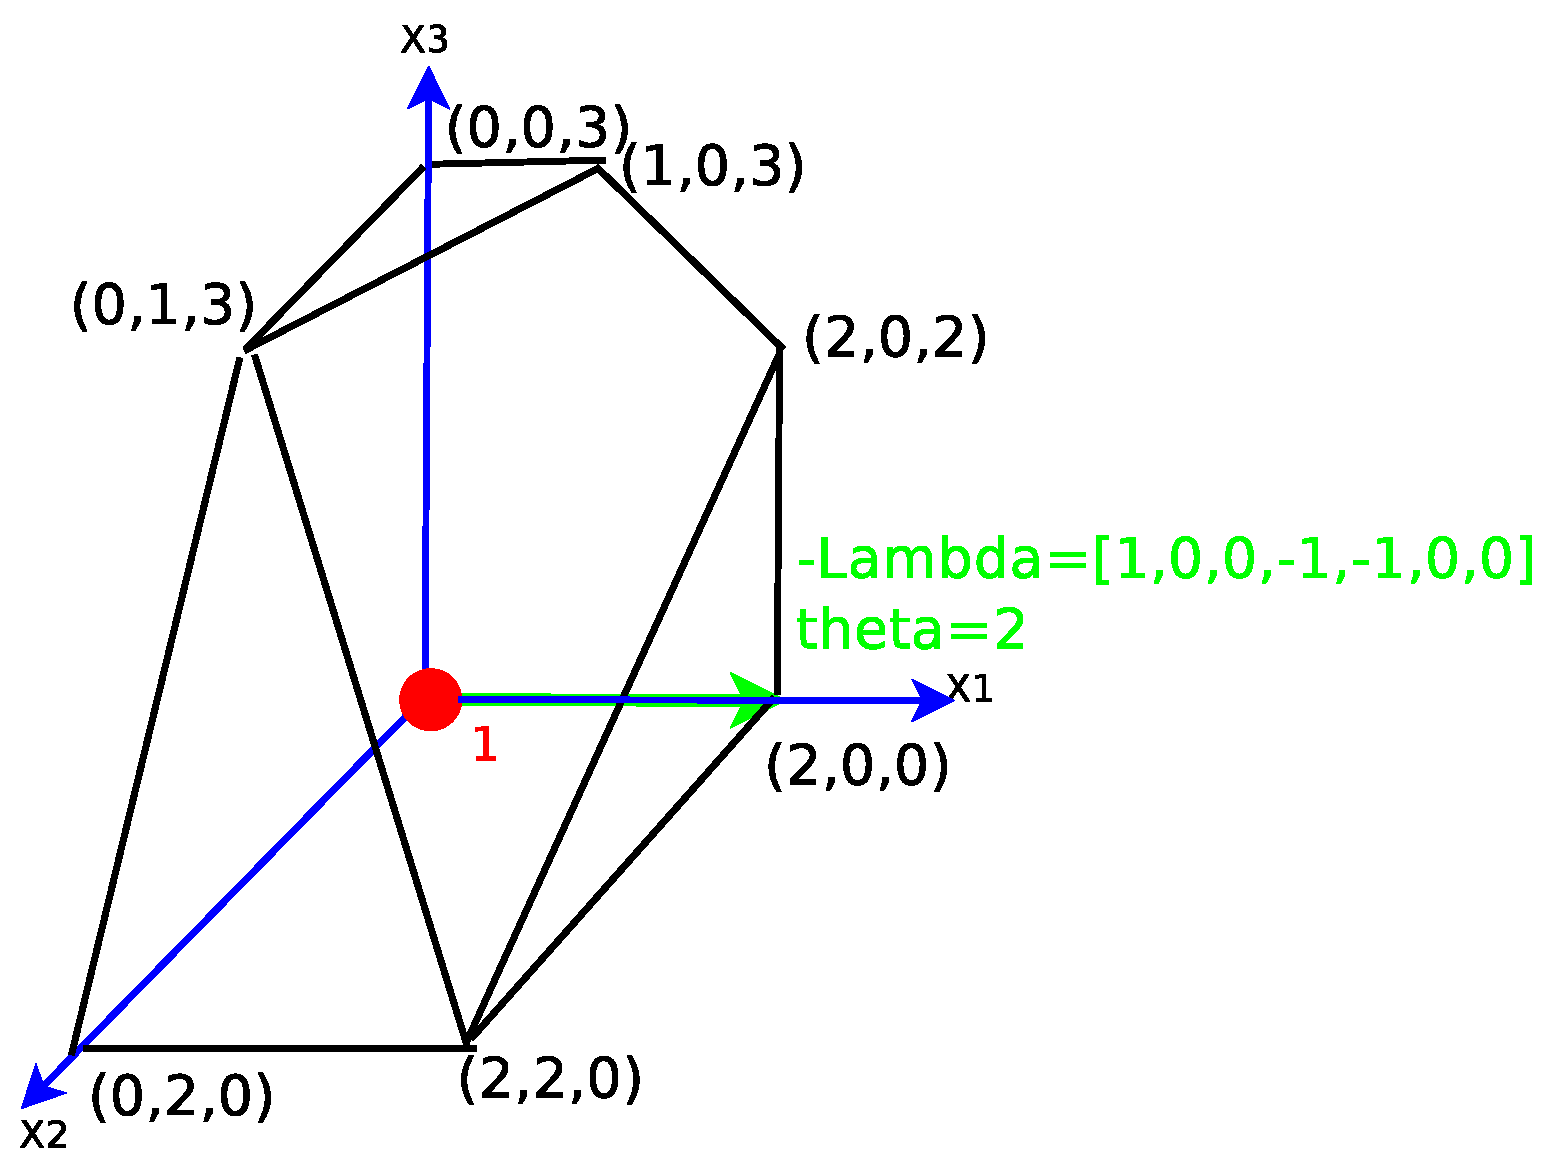
\includegraphics[width=1.4in] {L8-LPexample3Dstep1.eps}
%\end{figure}


\begin{small}
\begin{table}
{
\begin{tabular}{r|rrrrrrr}\hline 
  & $x_1$ & $x_2$ & $x_3$ & {$x_4$} & \textcolor{blue}{$x_5$} & \textcolor{blue}{$x_6$} & \textcolor{blue}{$x_7$}\\
\hline
 -z= 0 & $\overline{c_1}$=$-\frac{3}{4}$ & $\overline{c_2}$=150 & $\overline{c_3}$=$-\frac{1}{50}$ & $\overline{c_4}$=6 & $\overline{c_5}$=0 & $\overline{c_6}$=0 & $\overline{c_7}$=0 \\
 \hline
 $\mathbf{x_{B1}} = b_1'$=0 & \textcolor{red}{$\frac{1}{4}$} & -60 & $-\frac{1}{25}$ & 9 & \textcolor{blue}{1} & \textcolor{blue}{0} & \textcolor{blue}{0} \\
 $\mathbf{x_{B2}} = b_2'$=0 &  $\frac{1}{2}$ & -90 & $-\frac{1}{50}$ & 3 &  \textcolor{blue}{0}  &  \textcolor{blue}{1} & \textcolor{blue}{0} \\
 $\mathbf{x_{B3}} = b_3'$=1 &  0 & 0 & 1 & 0 &  \textcolor{blue}{0} & \textcolor{blue}{0} & \textcolor{blue}{1} \\
\hline
\end{tabular}
} %{}%
\end{table}
\end{small}

\begin{itemize}
 \item Same as step 1. A cycle! 
 \end{itemize}


}

\frame{
\frametitle{Bland rule to avoid cycling}
\begin{itemize}
 \item 
Cycling: If a sequence of pivots starting from some basic feasible solution ends up at the exact same basic feasible solution, then we refer to this as “cycling.” If the simplex method cycles, it can cycle forever.

\item
Bland indexing rule: \begin{enumerate}
             \item
choose $ \mathbf{a}_j$ to enter: $j=\min\{j: \bar{c_j} \leq 0\}$. \\
\item
             choose $ \mathbf{a}_i$ to exit: choose the smallest $l$ to break ties.
            \end{enumerate}
\end{itemize}
Let's see how Bland rule works for this example. 
}


\frame{
\frametitle{ Step 5'. }

%\begin{figure}
% 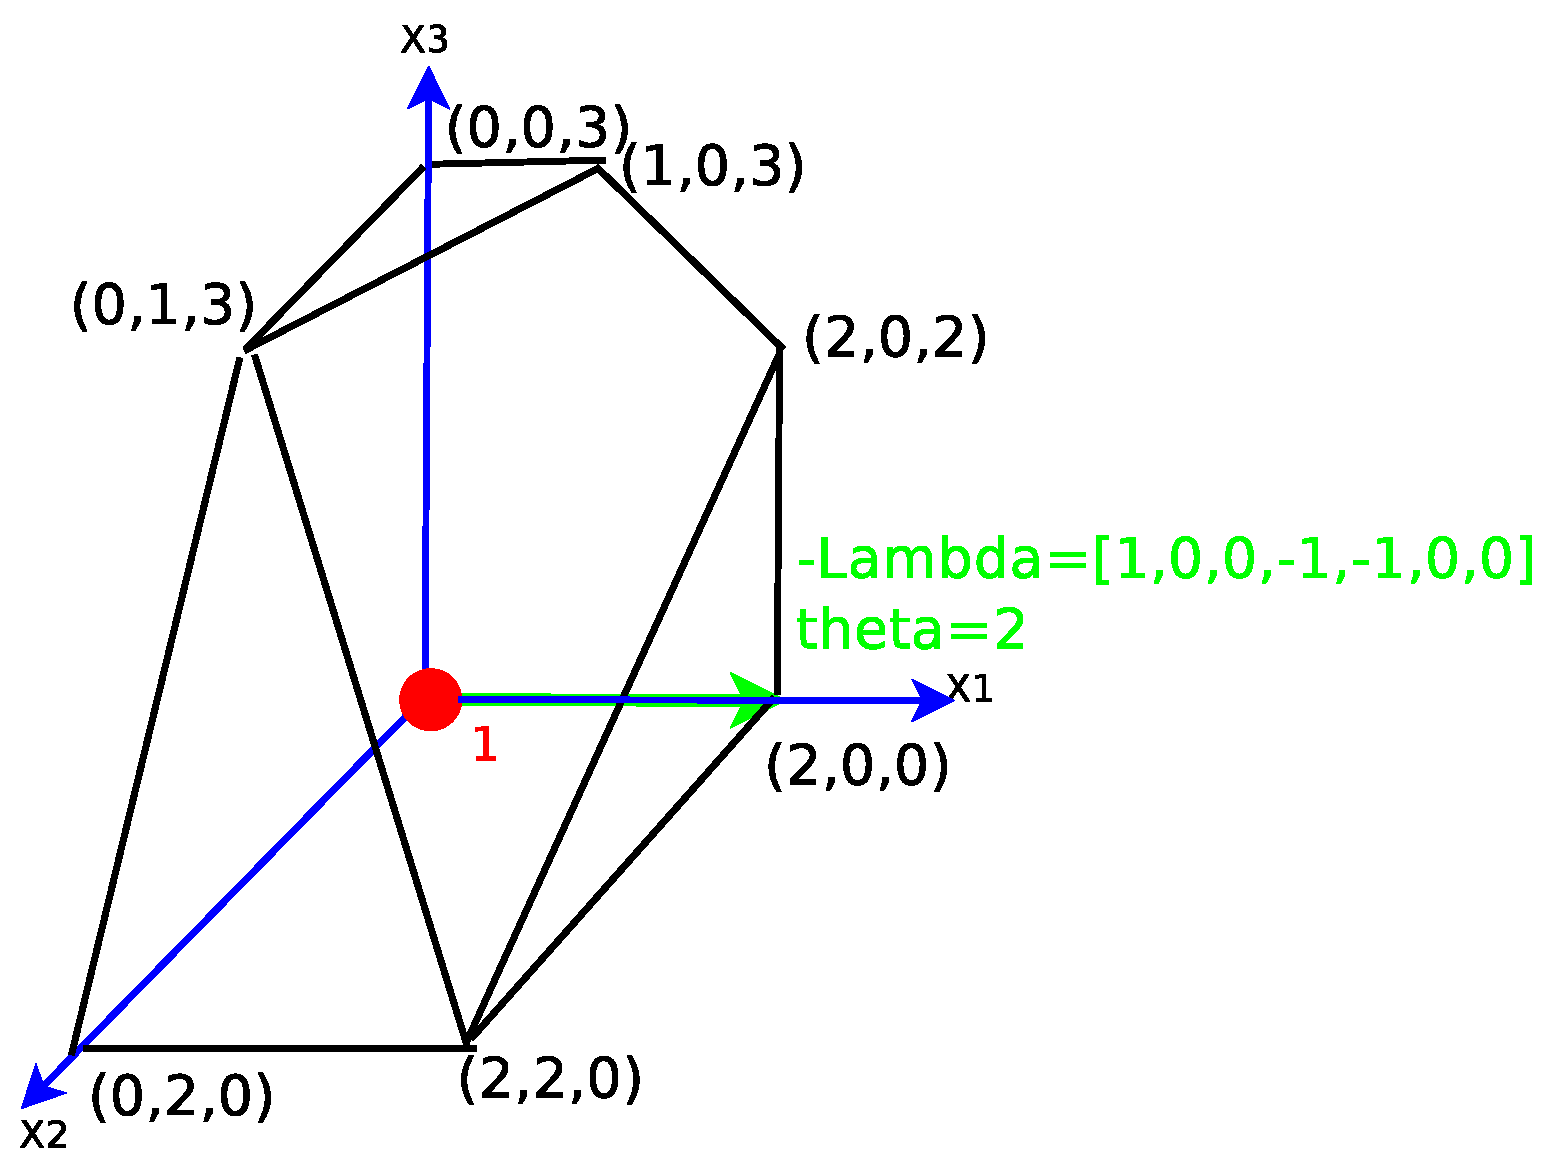
\includegraphics[width=1.4in] {L8-LPexample3Dstep1.eps}
%\end{figure}


\begin{small}
\begin{table}
{
\begin{tabular}{r|rrrrrrr}\hline 
  & $\textcolor{black}{x_1}$ & $\textcolor{black}{x_2}$ & $\textcolor{blue}{x_3}$  & \textcolor{blue}{$x_4$} & \textcolor{black}{$x_5$} & \textcolor{black}{$x_6$} & \textcolor{blue}{$x_7$}\\
\hline
 
 -z= 0 & $\overline{c_1}$=$-\frac{1}{2}$ & $\overline{c_2}$=120 & $\overline{c_3}$=0 & $\overline{c_4}$=0 & $\overline{c_5}$=-1 & $\overline{c_6}$=1 & $\overline{c_7}$=0 \\
 \hline
 
 $\mathbf{x_{B1}} = b_1'$=0 & $-\frac{125}{2}$ & 10500    & \textcolor{blue}{1} &  \textcolor{blue}{0}  & {50}   & -150 & \textcolor{blue}{0} \\
 
 $\mathbf{x_{B2}} = b_2'$=0 &  $-\frac{1}{4}$  & 40 & \textcolor{blue}{0} &  \textcolor{blue}{1}    & $\frac{1}{3}$  &  $-\frac{2}{3}$& \textcolor{blue}{0} \\
 
 $\mathbf{x_{B3}} = b_3'$=1 & \textcolor{red}{ $\frac{125}{2}$ } & 10500 & \textcolor{blue}{0} &  \textcolor{blue}{0}   &  50   & 150 & \textcolor{blue}{1} \\
\hline
\end{tabular}
} %{}%
\end{table}
\end{small}

\begin{itemize}
 \item Basis (in blue): $\mathbf{B =\{ a_3, a_4, a_7 \} }$.
 \item Solution: $\mathbf{x = [ x_B, x_N ] = [ B^{-1}b, 0] }= [ 0, 0, 0, 0, 0, 0, 1 ]$. 
 \item Pivoting (in red): choose $\mathbf{a_1}$ to enter basis since $\overline{c_1} = -\frac{1}{2} < 0$; 
 choose $\mathbf{a_7}$ to exit since $\theta = \min_{\mathbf{a}_i \in \mathbf{B}, \lambda_{i}>0} \frac{b'_i}{\lambda_{i} } = \frac{b'_3}{\lambda_{3} }= \frac{2}{125}$.
    \item Here, the corresponding $\mathbf{\lambda}$ is stored in the $1$-st column (Why? the basis $\mathbf{B}$ forms an identity matrix.)
 \item  Note: $\theta \neq 0$. Escaped from the cycle!
\end{itemize}

}










\end{document}
